\documentclass{standalone}
\usepackage{tikz}
\usetikzlibrary{shapes, calc, shapes, arrows}
\usepackage{amsmath,amssymb}
\usepackage{xcolor}
\definecolor{lightblack}{HTML}{333333}
\begin{document}
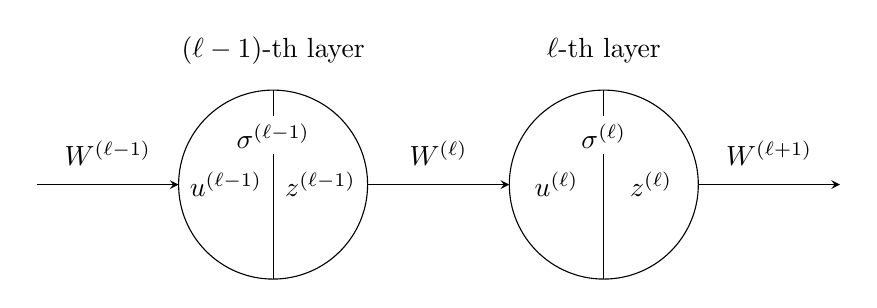
\begin{tikzpicture}
    \def\radius{1.2}
    \def\x{4.2}

    \node (O) at (0, 0) {};
    \draw (O) circle [radius=\radius];
    \draw (0, -\radius) -- (0, .32 * \radius);
    \draw (0, .73 * \radius) -- (0, \radius);

    \node (west) at (-\radius, 0) {};
    \node (east) at (\radius, 0) {};

    \node at (0, .62) {$\sigma^{(\ell)}$};
    \node at (0, 1.7) {$\ell$-th layer};
    \node at ($(O)!0.5!(west)$) {$u^{(\ell)}$};
    \node at ($(O)!0.5!(east)$) {$z^{(\ell)}$};
    \node at (0.5 * \x, 0.4) {$W^{(\ell + 1)}$};
    \node at (-0.5 * \x, 0.4) {$W^{(\ell)}$};


    \node (westnext) at ({\x -\radius}, 0) {};
    \draw[-stealth] (east.center) -- (westnext.center);

    \node (Oprev) at (-\x, 0) {};
    \draw (Oprev) circle [radius=\radius];
    \draw (-\x , -\radius) -- (-\x, .32 * \radius);
    \draw (-\x, .73 * \radius) -- (-\x, \radius);

    \node (westprev) at ({-\x - \radius}, 0) {};
    \node (eastprev) at ({-\x + \radius}, 0) {};

    \node at (-\x, .62) {$\sigma^{(\ell - 1)}$};
    \node at (-\x, 1.7) {$(\ell - 1)$-th layer};
    \node at ({-\x - 0.5 * \radius}, 0) {$u^{(\ell - 1)}$};
    \node at ({-\x + 0.5 * \radius}, 0) {$z^{(\ell - 1)}$};
    \draw[-stealth] (eastprev.center) -- (west.center);

    \node (eastprevprev) at ({-2 * \x + \radius}, 0) {};
    \draw[-stealth] (eastprevprev.center) -- (westprev.center);

    \node at (-1.5 * \x, 0.4) {$W^{(\ell - 1)}$};
\end{tikzpicture}
\end{document}
